%%%%%%%%%%%%%%%%%%%%%%%%%%%%%%%%%%%%%%%%%%%%%%%%%%%%%%%%%%%%%%%%%%%%%%%%%%%%%%%%
% Template for USENIX papers.
%
% History:
%
% - TEMPLATE for Usenix papers, specifically to meet requirements of
%   USENIX '05. originally a template for producing IEEE-format
%   articles using LaTeX. written by Matthew Ward, CS Department,
%   Worcester Polytechnic Institute. adapted by David Beazley for his
%   excellent SWIG paper in Proceedings, Tcl 96. turned into a
%   smartass generic template by De Clarke, with thanks to both the
%   above pioneers. Use at your own risk. Complaints to /dev/null.
%   Make it two column with no page numbering, default is 10 point.
%
% - Munged by Fred Douglis <douglis@research.att.com> 10/97 to
%   separate the .sty file from the LaTeX source template, so that
%   people can more easily include the .sty file into an existing
%   document. Also changed to more closely follow the style guidelines
%   as represented by the Word sample file.
%
% - Note that since 2010, USENIX does not require endnotes. If you
%   want foot of page notes, don't include the endnotes package in the
%   usepackage command, below.
% - This version uses the latex2e styles, not the very ancient 2.09
%   stuff.
%
% - Updated July 2018: Text block size changed from 6.5" to 7"
%
% - Updated Dec 2018 for ATC'19:
%
%   * Revised text to pass HotCRP's auto-formatting check, with
%     hotcrp.settings.submission_form.body_font_size=10pt, and
%     hotcrp.settings.submission_form.line_height=12pt
%
%   * Switched from \endnote-s to \footnote-s to match Usenix's policy.
%
%   * \section* => \begin{abstract} ... \end{abstract}
%
%   * Make template self-contained in terms of bibtex entires, to allow
%     this file to be compiled. (And changing refs style to 'plain'.)
%
%   * Make template self-contained in terms of figures, to
%     allow this file to be compiled. 
%
%   * Added packages for hyperref, embedding fonts, and improving
%     appearance.
%   
%   * Removed outdated text.
%
%%%%%%%%%%%%%%%%%%%%%%%%%%%%%%%%%%%%%%%%%%%%%%%%%%%%%%%%%%%%%%%%%%%%%%%%%%%%%%%%

%%% Minor updates for SOUPS 2019 by Michelle Mazurek
%%% Minor updates for SOUPS 2022 by Rick Wash

\documentclass[letterpaper,twocolumn,10pt]{article}
\usepackage{usenix2022_SOUPS}

% to be able to draw some self-contained figs
\usepackage{tikz}
\usepackage{amsmath}

% inlined bib file
\usepackage{filecontents}

%-------------------------------------------------------------------------------
\begin{filecontents}{\jobname.bib}
%-------------------------------------------------------------------------------
@Book{arpachiDusseau18:osbook,
  author=      {Arpaci-Dusseau, Remzi H. and Arpaci-Dusseau Andrea C.},
  title=       {Operating Systems: Three Easy Pieces},
  publisher=   {Arpaci-Dusseau Books, LLC},
  year=        2015,
  edition=     {1.00},
  note=        {\url{http://pages.cs.wisc.edu/~remzi/OSTEP/}}
}
@InProceedings{waldspurger02,
  author=      {Waldspurger, Carl A.},
  title=       {Memory resource management in {VMware ESX} server},
  booktitle=   {USENIX Symposium on Operating System Design and
                  Implementation (OSDI)},
  year=        2002,
  pages=       {181--194},
  note=        {\url{https://www.usenix.org/legacy/event/osdi02/tech/waldspurger/waldspurger.pdf}}
  }
@inproceedings {pearman,
author={Sarah Pearman and Shikun Aerin Zhang and Lujo Bauer and Nicolas Christin and Lorrie Faith Cranor},
title={Why people (don{\textquoteright}t) use password managers effectively},
booktitle={Fifteenth Symposium on Usable Privacy and Security (SOUPS 2019)},
year={2019},
isbn={978-1-939133-05-2},
address={Santa Clara, CA},
pages={319--338},
url={https://www.usenix.org/conference/soups2019/presentation/pearman},
publisher={USENIX Association},
month=aug,
}
@inproceedings {pwdhash,
author={Blake Ross and Collin Jackson and Nick Miyake and Dan Boneh and John C Mitchell},
title={Stronger Password Authentication Using Browser Extensions},
booktitle={14th USENIX Security Symposium (USENIX Security 05)},
year={2005},
address={Baltimore, MD},
url={https://www.usenix.org/conference/14th-usenix-security-symposium/stronger-password-authentication-using-browser-extensions},
publisher={USENIX Association},
month=jul,
}
@techreport{ssp,
  author={Alan H. Karp}
  title="Site-Specific Passwords",
  year=2002,
  number={HPL-2002-39},
  url={https://www.hpl.hp.com/techreports/2002/HPL-2002-39R1.pdf}
}
@inproceedings{10principles,
author={Yee, Ka-Ping},
title={User Interaction Design for Secure Systems},
year={2002},
isbn={3540001646},
publisher={Springer-Verlag},
address={Berlin, Heidelberg},
booktitle={Proceedings of the 4th International Conference on Information and Communications Security},
pages={278?290},
numpages={13},
series={ICICS '02}
url={http://zesty.ca/pubs/icics-2002-uidss.pdf}
}
@inproceedings{zxcvbn,
author={Wheeler, Daniel Lowe},
title={Zxcvbn: Low-Budget Password Strength Estimation},
year={2016},
isbn={9781931971324},
publisher={USENIX Association},
address={USA},
booktitle={Proceedings of the 25th USENIX Conference on Security Symposium},
pages={157?173},
numpages={17},
location={Austin, TX, USA},
series={SEC'16}
}
@phdthesis{oesch,
author={Oesch, Timothy},
title={An Analysis of Modern Password Manager Security and Usage on
Desktop and Mobile Devices},
year=2021,
school={University of Tennessee},
url={https://trace.tennessee.edu/utk_graddiss/6670/}
}
@inproceedings{silver2014password,
  title={Password managers: Attacks and defenses},
  author={Silver, David and Jana, Suman and Boneh, Dan and Chen, Eric and Jackson, Collin},
  booktitle={23rd $\{$USENIX$\}$ Security Symposium ($\{$USENIX$\}$ Security 14)},
  pages={449--464},
  year={2014}
}
\end{filecontents}


%-------------------------------------------------------------------------------
\begin{document}
%-------------------------------------------------------------------------------

%don't want date printed
\date{}

% make title bold and 14 pt font (Latex default is non-bold, 16 pt)
\title{\Large \bf SitePassword: A Password Calculator/Manager}

% if you leave this blank it will default to a possibly ugly attempt 
% to make the contents of the \author command below into a string
\def\plainauthor{Author name(s) for PDF metadata. Don't forget to anonymize for submission!}

%for single author (just remove % characters)
\author{
{\rm Alan H.\ Karp}\\
Independent
% copy the following lines to add more authors
% \and
% {\rm Name}\\
%Name Institution
} % end author

\maketitle
\thecopyright

%-------------------------------------------------------------------------------
\begin{abstract}
%-------------------------------------------------------------------------------
Most password managers store passwords so you don't have to remember them.  That choice imposes costs on the company providing the password manager and risks on its users.  Another option is to calculate passwords as they are needed.  SitePassword is such a calculator that provides all the key features that users want in their password manager -- remembering of metadata, synchronization across machines, and autofill capability.
\end{abstract}


%-------------------------------------------------------------------------------
\section{Introduction}\label{intro}
%-------------------------------------------------------------------------------

"Dealing with passwords is awful" is a statement few would disagree with.  Password managers make the situation less awful, improving both security and usability.  Basically, they make it easier for you to have a different, strong password for every site.  Of course, users care at least as much about ease of use, trust in the the password manager, and the ability to get their passwords from any of their machines or when using a friend's machine as they do the strength of their passwords.

There are two kinds of password managers.  The vast majority of them remember passwords and other metadata, such as userids.   They  make the stored passwords available from any machine by using  encrypted databases and cloud storage.

Remembering passwords adds cost for the company providing the password manager for it to manage user accounts and to pay for the necessary cloud storage.  It imposes risks on the user because the stored passwords can be stolen.  It has also happened that companies have dropped support for their password databases,\footnote{https://www.remembear.com/} leaving users in the lurch.

The second kind, password calculators, doesn't need to store passwords.  They combine a super password with other data to calculate a strong password for a website when you need to login.  SitePassword is a password calculator designed for usability and security that supports all the features users want.  Usability features are discussed in Section \ref{sec:usability}.

SitePassword remembers your settings for each site and synchronizes them across your machines without the need for user accounts or cloud storage.  It does that by putting the metadata in bookmarks, which virtually all browsers synchronize across machines.  Using bookmarks makes the settings available on machines that cannot install the extension, such as mobile devices. The security aspects of this choice are covered in Section \ref{sec:security}.

Unlike most password calculators, SitePassword provides features usually found only in password managers that store passwords.  In addition to synchronizing across machines, SitePassword finds and autofills both userid and password fields and includes a web page for use on machines where it is unavailable.  The Appendix compares SitePassword to other password calculators in the Chrome Store.

%-------------------------------------------------------------------------------
\section{SitePassword Overview}\label{sec:overview}
%-------------------------------------------------------------------------------

SitePassword is an extension that runs in Chromium browsers.\footnote{Brave, Chrome, Edge, and Opera.  Firefox is not a pure Chomium Browser.}  It has three components.  The popup, with the user interface shown in Figure~\ref{fig:popup}, is where the user provides the necessary metadata.  A content script running on the page with the login form is responsible for finding the userid and password fields on the page and filling them in on request.  A service worker manages the metadata and calculates the site password when the content script asks for it.  

\begin{figure}
\begin{center}
  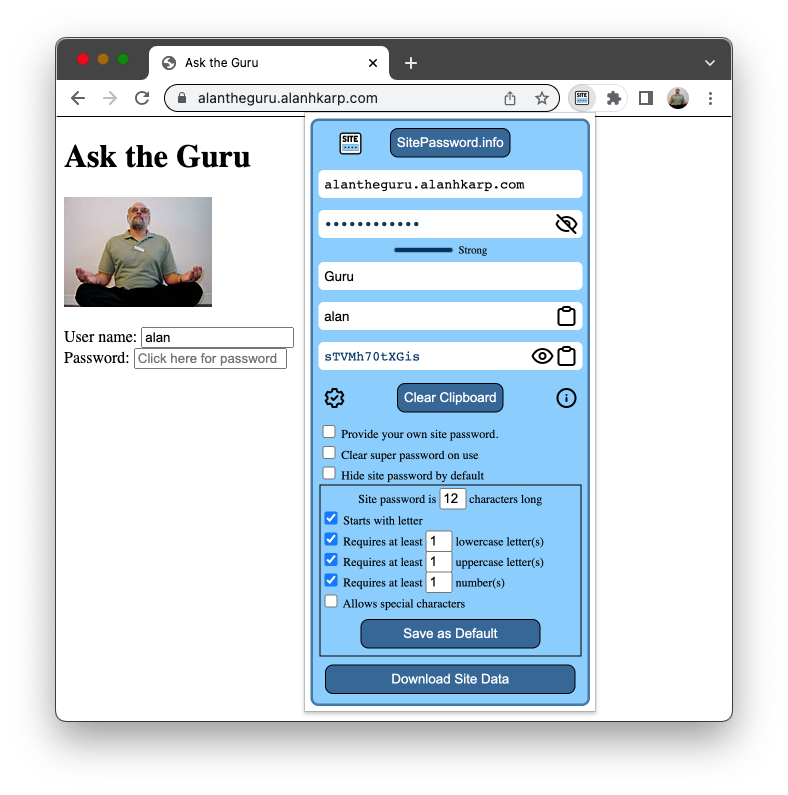
\includegraphics[scale=0.30]{soupsfig1.png}
\end{center}
\caption{\label{fig:popup} The SitePassword popup showing all available
options. }
\end{figure}

\begin{figure}
\begin{center}
  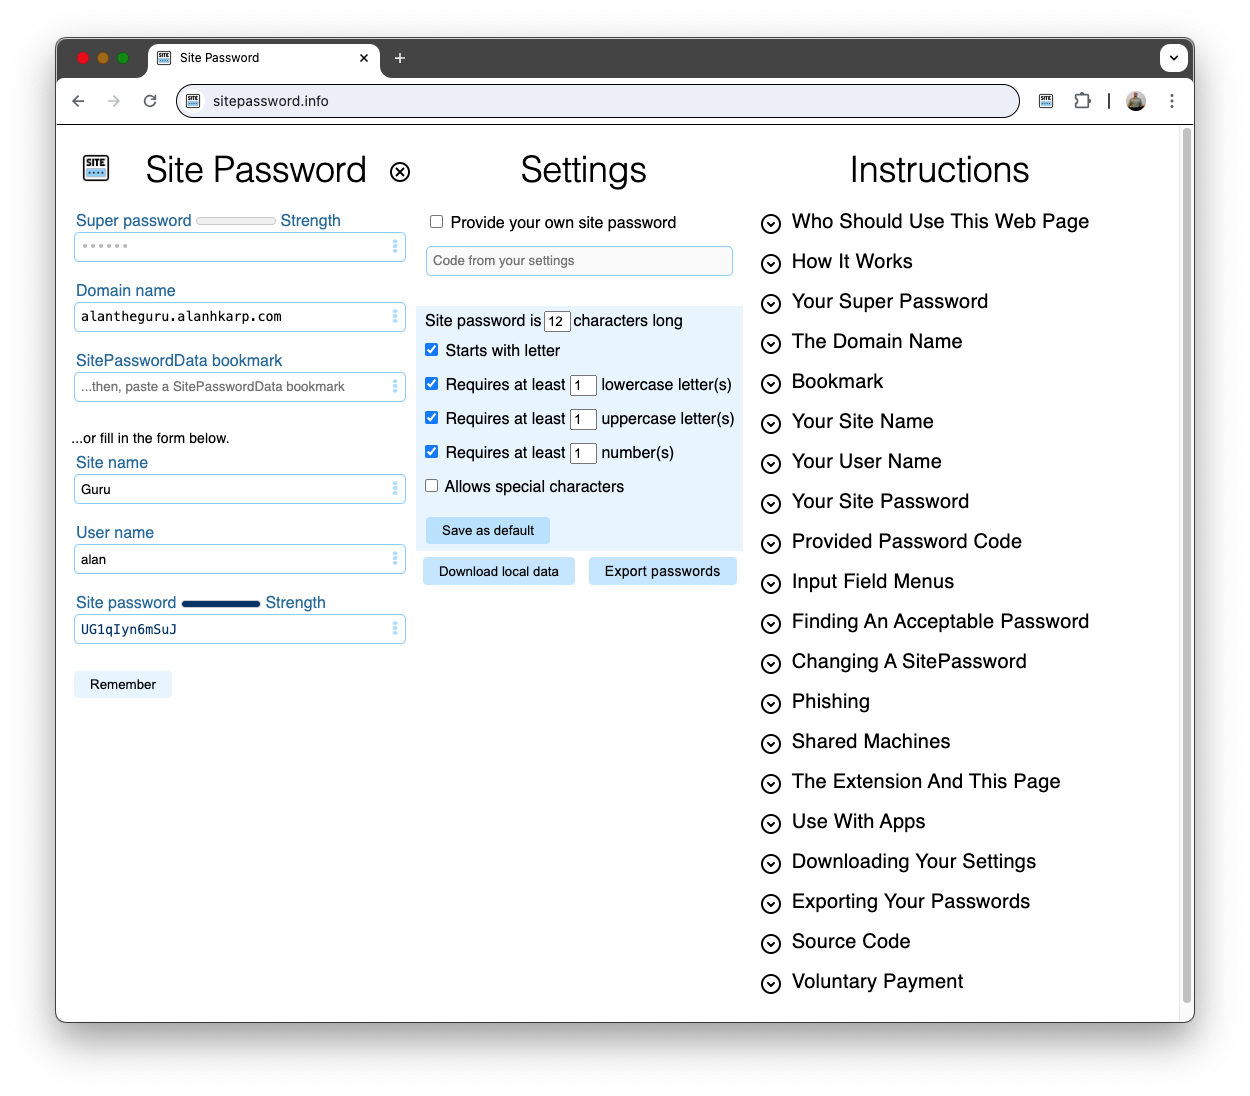
\includegraphics[scale=0.30]{soupsfig2.png}
\end{center}
\caption{\label{fig:webpage} The SitePassword web page showing all available options and the table of contents of the instructions.  Note that the calculated password is the same as in Figure 1. }
\end{figure}

When the user first encounters a page with a login form at a given domain, the password field contains a placeholder {\em Click SitePassword}.  Clicking the SitePassword icon opens the popup.  As you fill out the form the site password field updates on every keystroke, making it clear how uncorrelated the passwords are.

As you  mouse over to the password field, your userid gets filled in and the placeholder changes to say {\em Click here for password}.  Click and your password gets filled in.  When returning to that login page on any machine that synchronizes your bookmarks and has the extension installed, you only need to click on the password field.  The result is that using SitePassword is even easier than typing the same, weak password for every site.

SitePassword also includes a web page, shown in Figure~\ref{fig:webpage}, that can be used to get your passwords when the extension is not available, such as on your mobile devices.  You don't even have to remember your settings if you synchronize bookmarks to the device.  You can paste the corresponding bookmark into the form.  

You can also download a nicely formatted table of your settings that you can print for times when your bookmarks are not available.  Losing this piece of paper adds only a small amount of vulnerability as discussed in Section~\ref{sec:security}.

%-------------------------------------------------------------------------------
\section{Usability Considerations}\label{sec:usability}
%-------------------------------------------------------------------------------

People who don't use a password manager often give usability as the main reason~\cite{pearman}.  SitePassword was designed to be as usable as a simple game.  Each step should be obvious; you should be able to experiment without worrying about breaking something; warnings make clear what next steps to take.  Although SitePassword comes with extensive instructions, as shown in Figure 2, the hope is that they won't be needed.

A very simple way to guide the user is to put the browser focus on the field that should be filled in next. Another is to disable fields until they are ready for user interaction.  For example, the settings that get stored are indexed by the domain name and associated with the nickname for the site. One choice would be to present an error message when the user tries to remember the settings without providing this information.  Instead, the {\em Remember Settings} button on the web version is only enabled after that information is available.

Another way to help the user is to put the information the user needs where the user is looking.  An example is the placeholder put in the password field of the login form. More extensive information is provided by tooltips, which also serve as a backup in cases when the placeholder isn't visible.

Websites often have rather specific password rules, such as how many upper case letters, numbers, and special case characters are needed and even which ones are acceptable.  The users only involvement in getting a valid site password is in filling out the form in the popup to specify the rules.  SitePassword automatically finds a suitable password by continually hashing until one is found, stopping after 1,000 tries.  While that could happen by chance, the most frequent cause is incompatible settings, such as asking for more numbers than the specified length of the password.  If that's not the case, trying again with a different nickname for the site will find a valid password with high probability.  No failure has occurred in a decade's use of this algorithm.

There are times when you need to type the site password manually.  The most common case is logging into an app on a smart TV.  In addition, it is possible that SitePassword won't find the password field on a page that has disabled pasting.  Hence, it is important to choose a readable font that doesn't make, for example, lower case l (ell) look like upper case I (eye).\footnote{An earlier version did not follow this advice, resulting in the author needing several tries to log into Netflix on his new smart TV.} 
 
\begin{figure}
\begin{center}
  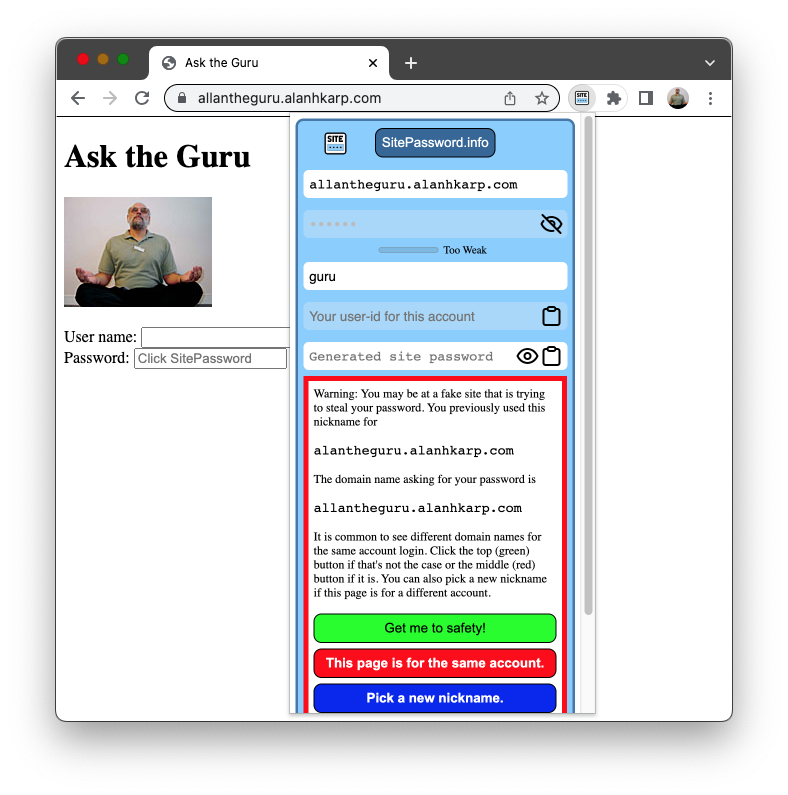
\includegraphics[scale=0.30]{soupsfig3.png}
\end{center}
\caption{\label{fig:phishing} The SitePassword phishing warning. }
\end{figure}

Phishing is a threat that SitePassword is in a position to warn about, but too many websites make it ambiguous by using multiple domain names for logging into the same account.  Unfortunately, it is virtually impossible to use the domain name to distinguish phishing from a legitimate use of a different domain name.  For example, are the domain names in Figures~\ref{fig:popup} and~\ref{fig:phishing} for the same account?  You can't use the trailing part of the domain name because alanhkarp.com might be providing these domain names as a service to independent parties.  Perhaps allan is attempting to phish users of alan's website.

The fact that most phishing warnings are spurious leaves two choices.  Either ignore them or explain them.  SitePassword made the latter choice in the hope that the explanation shown in Figure~\ref{fig:phishing} suffices.  

People often have different personas.  For example, you may have a machine that everyone in your family uses.  Everybody probably uses the same credentials for your streaming services but individual credentials for social media accounts.  Chromium browsers provide {\em Profiles} for this purpose.  Each profile gets its own browser settings, which includes bookmarks.  You get personas for free because SitePassword uses bookmarks to hold your settings.

One question is how you are going to remember the URL to use when you want a password when you're visiting a friend's house.  One thing that might help you remember is the title on the popup, which shows the URL and is a link to the page.  Whether or not that's sufficient is an open questions.

%-------------------------------------------------------------------------------
\section{Security Considerations}\label{sec:security}
%-------------------------------------------------------------------------------

A guiding principle is that a system cannot be secure if users are not aware of the implications of their actions.  To that end, the SitePassword user experience is based on 10 Principles for a Secure UX~\cite{10principles}.  For one, SitePassword makes the easy way the secure way, as noted in Section~\ref{sec:overview}.  It also requires a click on the password field both to avoid a family of attacks~\cite{silver2014password} and to give the user a sense of control.  Leaving a password on the clipboard is not good practice, so SitePassword indicates when that might be the case.  Finally, potential phishing results in a warning as shown in Figure~\ref{fig:phishing}.

Of course, that's not enough.  It's also necessary to keep the user informed.  To that end, SitePassword provides a strength meter for the super password and uses the same colors for the site password in case a generated one is weak.

Other protections aren't visible to the user.  The user's super password is never stored.  It is kept in session memory, a transient space only available to the extension for the duration of the browser session.  The callback that fills in the password is only registered on visible password elements, making clickjacking more difficult.  If that element is in an iframe, the domain name of that iframe is used to select the metadata used to calculate the site password.  Using the userid and site's nickname in the computation provides salt to protect the super password from pre-image attacks.

Some decisions slightly weaken security to give a big gain in usability.  For example, the site password is visible by default to increase the user's trust in the generated passwords.\footnote{Besides, it's cool watching it change as you type.}  While users have the option to change the default, any risk is mitigated by the fact that you only open the popup rarely -- to set up a new password, to enter your super password at the start of a browser session, or when you need to paste your site password.  Another decision was choosing a default site password length of 12 because some websites do not accept longer ones, although that has become less of an issue in recent years. 

The main decision that weakens security is using unencrypted bookmarks to store your settings.   The benefits are huge in that there's no need for user accounts or cloud storage, the settings are available on your mobile devices that can't install the extension, support for personas is provided by browser profiles, and the risk is low.  All an attacker gains is the sites you log into and your userids at those sites.  That's not nothing, but knowing that gives no hint of either your super or site passwords.

There are two reasons not to encrypt.  First, the user selects to the bookmark by domain name when pasting it into the web form, which means a key piece of data must be in the clear.  Second, the user might have different super passwords for different classes of web sites.  It wasn't deemed worth the complication just to protect your userids, which are often easy to guess.

There are also mitigating factors.  It is hard to get to the bookmarks from a web page, so malware on your machine is the main threat.  Such malware is likely to cause bigger problems than exposing your SitePassword settings.

The biggest threat you face is an offline attack against your super password.  Say that you create an account at a rogue site.  The site owner knows your userid and site password and can probably guess your nickname for the site.  The site owner can now mount an offline guessing attack against your super password.

There are three mitigations.  First is choosing a strong super password.  According to zxcvbn~\cite{zxcvbn}, which is used for the password strength meter, it would take 30 days to guess a 12-character password at a $10^6$ guesses per second.  The second is that SitePassword hashes a minimum of 100 times before producing a site password, increasing the attackers work factor by that amount.  The third is up to the user.  Nothing says you can have only one super password.  You could have one for banking and health accounts, a second for subscriptions, and a third for sketchy sites.  This choice is not readily available for password managers that store your passwords. 

%-------------------------------------------------------------------------------
\section{Related Work}\label{sec:related}
%-------------------------------------------------------------------------------

There are a number of reviews~\cite{oesch} of the kind of password manager that stores passwords, so this section only reviews password calculators.  The Appendix has notes on all the password managers in the Chrome store that provide password manager features.

An early very simple calculator~\cite{ssp} hashed the user's super password with a user selected nickname for the site to produce a password that the user would copy and paste into the password field.  It was later adapted into the HP Antiphishing Toolbar for Internet Explorer, which added many of the features of a modern password manager.

PwdHash~\cite{pwdhash} combines the user's password with the domain name of the page.  Its key advantage is familiarity; the user simply types into the login form's password field.  SitePassword trades this familiarity for the simplicity of just clcking on the password field.  The PwdHash algorithm means that you get different password if the site uses different domain names for the same account, a problem SitePassword solves by associating the settings with a user chosen nickname for the site.  PwdHash's greatest strength is the protection it affords when typing passwords into pages with malicious JavaScript, which is not a problem for SitePassword because the user only types into the popup.


%-------------------------------------------------------------------------------
\section{Future Work}\label{sec:future}
%-------------------------------------------------------------------------------

There is still work to be done.  A user study would identify any glitches in the user experience.  A comprehensive security review of both the design and the code should also be done.  Unfortunately, there is no funding to support either of them.  In lieu of a user study, SitePassword is only available to those who know its URL in the Chrome Store.  The hope is that early users will provide sufficient feedback.  Informal discussions with a number of security experts has confirmed the validity of several aspects of the design.

Work has started on porting SitePassword to both Firefox and Safari, 
but there is no plan to create an app for mobile devices because of 
existing security problems~\cite{oesch} on those platforms.

%-------------------------------------------------------------------------------
\section{Conclusions}\label{sec:conclusions}
%-------------------------------------------------------------------------------

SitePassword is a full-featured password manager that includes the features people want most -- ease of use, trustworthiness, remembering of metadata, and availability of passwords across devices.  Because it doesn't require user accounts or cloud storage, it is free.  It is also open source, allowing a company to produce a version with corporate branding.

%-------------------------------------------------------------------------------
\section*{Acknowledgements}\label{sec:acks}
%-------------------------------------------------------------------------------

The author would like to thank Dale Schumacher for both providing a professional look and feel to the user interface, significant code improvements to the web version, and generally useful discussion.  Douglas Crockford provided significant feedback as an early adopter, and Jasvir Nagra provided guidance needed to make the content script work properly.  Useful input came from the Friam security group.

%-------------------------------------------------------------------------------
\bibliographystyle{plain}
\bibliography{\jobname}

\pagebreak

\onecolumn
%-------------------------------------------------------------------------------
\section*{Appendix}\label{sec:appendix}
%-------------------------------------------------------------------------------

There are a LOT of password managers in the Chrome extension store.  The majority store passwords, but there are a lot that calculate them.  I installed all of the following and attempted to use each one to figure out what features it supports.  Some of them I couldn't figure out how to make work; others didn't work at all.  Very few provided enough control to always generate a legal password.  Many of them were updated in the last two years even though very few had more than a dozen users.

Table~\ref{table:appendix} summarizes properties of the other password calculators in the Chrome store that have at least some password manager features.  The column headings are:

\begin{itemize}
\setlength\itemsep{0em}
\item Extension: The name of the extension to search in the Chrome store
\item Inputs: The values used to compute the password, settings include such things as the number of upper and lower case letters. 
\item M: Which values are remembered across invocations
\item S: If settings are synched across machines
\item R: If there is a way to conform to the site's password rules
\item O: If you can get your passwords if the extension isn't available
\item P: If you are warned of potential phishing
\item A: If you need an account
\item D: App for mobile devices
\item E: Use existing passwords
\end{itemize}



\begin{table}[b]
\label{table:appendix}
\caption{Comparison of password calculators}
\begin{tabular}{|l  |  |  p{0.6in}  | p{0.6in} | c | c | c | c | c |  c | c | c | p{2in}  |}
\hline
 Extension  & Inputs & Autofill & M & S & R & O & P  & A & D & E & Notes \\\hline
 SitePassword & super pw\newline site name\newline user name\newline settings & user name sitename & All & Y & Y & Y & Y  & N & N & Y & Settings include which special characters\\\hline
 MindYourPass &      &     &     &    &     &   &  &   Y & Y & Y & Can use biometrics\\\hline
\end{tabular}
\end{table}

\begin{itemize}
\item MindYourPass: uses cookies to store

%https://chrome.google.com/webstore/detail/mindyourpass-on-the-fly-p/ahnaknhjlbcofkaiapoldfkpacjegnme

\item OnePass: nickname  (domain name default)
 
%https://chrome.google.com/webstore/detailonepass-password-manager/emeedobobbobllpippjidhpiigoffbbj 

\item PasswordGenerator: nickname (domain name default)
 
%https://chrome.google.com/webstore/detail/password-generator/klfojgipmkdgfmikjfdhhkjlfeboaoij 

\item GenPass: nickname (domain name default)

%https://chrome.google.com/webstore/detailgenpass-strong-password-g/ocdpddbeogmhochlpfchdcjojhfljalg

\item Password Chameleon: nickname, not site address

%https://chrome.google.com/webstore/detailpassword-chameleon/ihgpfjkeignaegoghdopjncdahgilfnc

\item PasswordMaker: nickname, autofill, save username as a global, not per site

%https://chrome.google.com/webstore/detailpasswordmaker-org/fckpmekmkjglpmdcbfkchimdelcjiipd 

\item GMP:  nickname (called PIN), no phishing warning

%https://chrome.google.com/webstore/detailgmp/lghchjpnonkjgcofdgclcpnooaggdoje

\item PasswordMaker: nickname, autofill

%https://chrome.google.com/webstore/detailpasswordmaker/gnfjppomohbcojfccghjcgahfofgmgdn 

\item LessPass: 

%https://chrome.google.com/webstore/detaillesspass/lcmbpoclaodbgkbjafnkbbinogcbnjih

\item Amaranth: doesn't work but uses nickname

%https://chrome.google.com/webstore/detailamaranth-password-manager/hbkfmkahandehhbdlgbfhaeacecfeceo

\item Pure: nickname, autofill password, no phishing warning, no paste option, doesn't work with multiple password fields

%https://chrome.google.com/webstore/detailpure-password-manager/hadhkedhiabkdhjhcpcjcmojcaaldijm 

\item HashPass: nickname, no memory, no autofill

%https://chrome.google.com/webstore/detailhashpass/gkmegkoiplibopkmieofaaeloldidnko 

\item HashWord: domain name (can't edit) auto fill, no memory, different passwords for same account, moves password field into shadow root

%https://chrome.google.com/webstore/detailhashword/nkdpamnjhdjoncifjaoojhmfdmdknamo 

\item Entropass: nickname, autofill of password only if blank, hash includes userid, moves password field into shadow root

%https://chrome.google.com/webstore/detailentropass/andieidkfneadmcoolmlecilekpnclki 

\item SynthPass: autofill, can't find Schwab password field, no copy option, can't handle multiple password fields

%https://chrome.google.com/webstore/detailsynthpass/khkpfnickpejcjhajmkljfadcaegphkd 

\item PawHash: nickname, autofill, no copy option, autofills all password fields if multiples, doesn't remember nickname

%https://chrome.google.com/webstore/detailpawhash/adgekjfphhgngpdoklolpjenmgneobfg

\item SuperGenPass: bookmarklet, can't figure out how it works

%https://chrome.google.com/webstore/detailsupergenpass-for-google-c/bmmmhbgdbpnbfefmacdlbpfgegcibkjo 

\item OfflinePass: domain name, memory, no autofill

%https://chrome.google.com/webstore/detailoffline-pass/dohnghdcmkckopegdlbjagkpdcadapmd 

\item 
PersiPass: last 2 parts of domain name, amazon.co.uk comes out as co.uk

%https://chrome.google.com/webstore/detailpersipass/eajbmafhfoombigogdbioomechdcmiob 

\item ToughPassword: combines super password with selections from visual grid, no memory

%https://chrome.google.com/webstore/detailtough-password/gdkmnhfejfcgfckdbecheieeeklnilai 

\item PasswordAssistant: nickname, weak passwords, no memory

%https://chrome.google.com/webstore/detailpassword-assistant/fefgbdipgjhdeindoaggjgbogpelddhg

\item Crypto-Pass: nickname, no memory as a feature

%https://chrome.google.com/webstore/detailcrypto-pass/polodkmafdgpbmfnenjpccjpcnhnfenm 

\item SimplePasswords: nickname, remembers superpw, autofills password

%https://chrome.google.com/webstore/detailsimple-passwords/gmfjgamlejnjeldifhbhiahhjkddobnh 

\item Motornyy: autofill (didn't work), no memory

%https://chrome.google.com/webstore/detailmotornyy-passwords/oocaafogiegbgcnkghppklpaofnkjeob 

\item Nikagi: nickname, no memory

%https://chrome.google.com/webstore/detailnikagi/kkeiaegfmfbiiflklgkhlbjhhdiejimn

\item SaltedPass:  broken? I get the same password for all super passwords and domains

%https://chrome.google.com/webstore/detailsaltedpass/fkechapmoaignhmmmaifkkmjkmbmlcdk 

\item ReAnPro: can't figure out how to use it.

%https://chrome.google.com/webstore/detail/rean-pro/hieeechfngndnjbhffahmnagpiejjmnh 

\item sitePass: nickname, no memory, web page 404

%https://chrome.google.com/webstore/detailsitepass/knipommgdbefafccijppfjoiokhcedgn 

\item Passwords101: nickname, no memory, no autofill

%https://chrome.google.com/webstore/detailpasswords-101/iabacjkjeeoojogfgbdabjngagbajjgl 

\item Just1Password: nickname that looks like an email address, memory but not super password, includes part of domain name, alantheguru and allantheguru get the same password, amazon.com and amazon.co.uk don't

%https://chrome.google.com/webstore/detail/just1-password/kadnpfobnjcfechkibldpapjgolgpcbn 

\item MashPass: nickname, no memory, no autofill, no phishing warning

%https://chrome.google.com/webstore/detailmashpass/ifodomenmbgaimnbbomagcmedmdffkgj 

\item Vaultpass:  nickname, no memory, no autofill, no phishing warning

%https://chrome.google.com/webstore/detailvaultpass/ehihnbmbopnllneioglejhanemdgldpd
\end{itemize}

%%%%%%%%%%%%%%%%%%%%%%%%%%%%%%%%%%%%%%%%%%%%%%%%%%%%%%%%%%%%%%%%%%%%%%%%%%%%%%%%
\end{document}
%%%%%%%%%%%%%%%%%%%%%%%%%%%%%%%%%%%%%%%%%%%%%%%%%%%%%%%%%%%%%%%%%%%%%%%%%%%%%%%%

%%  LocalWords:  endnotes includegraphics fread ptr nobj noindent
%%  LocalWords:  pdflatex acks
